\chapter{Résultats}

Préalablement aux résultats acquis durant le stage, plusieurs étapes de mises au point (nottament sur lignées cellulaires de plasmocytes) 
ont été réalisées durant l'année 2024-2025. Les données ne seront pas présentés dans ce rapport, mais ont permis de valider la faisabilité 
de l'analyse des réarrangements \gls{vdj} via le protocole précédement décrit, sous-tenant quelques modifications, mais aussi de faire 
la lumière sur plusieurs difficultés.

\section{Difficultés techniques liées au protocole de séquençage FR3}

\subsection{Identification du segment V}

Une des premières difficultés rencontrées, inhérente à la nature du protocole utilisé, est l'incertitude sur l'identification 
du segment V. En raison de l'utilisation d'amorces ciblant la région \gls{fr}3, toujours dans l'optique d'analyser par les suite 
des \gls{adnc}, seuls 20 à 30 nucléotides sont séquencés en amont du réarrangement \gls{vdj}. Cette longueur ne permet pas à 
\textit{Vidjil} (ou tout autre outil d'analyse de réarrangements \gls{vdj}) de déterminer avec certitude le segment V utilisé 
(\autoref{fig:v-leader-fr3}). 
Une façon de palier à ce problème est de séquençer au diagnostic en utilisant des amorces ciblant la région \gls{fr}1 ou 
\textit{leader}, pour obtenir une séquence plus longue, et ainsi permettre à \textit{Vidjil} de déterminer le segment V utilisé. 
L'unicité de la région \gls{cdr}3 permettra ensuite de relier les clones identifiés sur les prélèvements de suivi.

\begin{figure}[H]
    \centering
    \begin{ttfamily}
        \begin{tabular}{@{}l@{}}
        \textbf{Clone IGHV1-3*04 // D3-16 // J3*02 (\textit{leader})} \\
        \colorbox{blue!20}{GCCAGGCCCCCGGTCAGAGGCTTGAGTGGATGGGCTGGGTCAACGGTGCCAGTGGCGACGCAAAATATTCACAGCAT} \\
        \colorbox{blue!20}{TTCCAGGGCGGAGTCACCATTACCAGGGACACTTCCGCGACTACAGCCTACATGGAACTGAGCAGCCTGAGATCTGAG} \\
        \colorbox{blue!20}{GACACGGCTGTCTATTACTGTGCGA}%
        \colorbox{green!20}{CTTATACC}AACACTTTTTGGTT%
        \colorbox{orange!20}{TGCTTTTGATATCTGGGGCCAAGGGACAA} \\
        \colorbox{orange!20}{TGGTCACCGTCTCCTCAG}GT \\
        \\
        \textbf{Clone IGHV3-30*08 // D3-16 // J3*02 (\gls{fr}3)} \\
        \textbf{
            \textcolor{red}{\faExclamationTriangle\  Gènes V équiprobables : IGHV3-66*02, IGHV3-7*02, IGHV3-30*08, IGHV4-34*12}
            } \\
        \colorbox{blue!20}{GACACGGCTGTCTATTACTGTGCGA}%
        \colorbox{green!20}{CTTATACC}AACACTTTTTGGTT%
        \colorbox{orange!20}{TGCTTTTGATATCTGGGGCCAAGGGACAA} \\
        \colorbox{orange!20}{TGGTCACCGTCTCCTCAG}GT
        \end{tabular}
    \end{ttfamily}
    \caption{Alignement de deux réarrangements clonaux identiques. Le premier clone (en haut) correspond à un réarrangement 
    complet séquencé en \textit{leader}, tandis que le second (en bas) commence au niveau de la région \gls{fr}3. 
    Les séquences en \colorbox{blue!20}{bleu} correspondent au segment V, en \colorbox{green!20}{vert} 
    au segment D, et les séquences en \colorbox{orange!20}{orange} correspondent au segment J.
    Les jonctions sont alignées pour souligner la différence de longueur des régions V.}
    \label{fig:v-leader-fr3}
\end{figure}
 
\subsection{Hypermutation somatique}

Il s'agit encore une fois d'une difficulté liée au protocole d'amplification \gls{fr}3 et à la nature des cellules d'interêt. 
En effet les plasmocytes constituent le stade le plus mature de la lignée lymphoïde B, et en ce sens sont donc les cellules où le 
réarrangement \gls{vdj} comporte le moins d'homologie avec les séquence germinales. La conséquence de ceci étant que dans certains 
cas, les amorces utilisées pour l'amplification \gls{fr}3 ne sont pas capables de se fixer sur les séquences \gls{vdj} mutées, et 
amplifier les réarrangements. L'utilisation d'amorces dégénérées permet de limiter ce problème sans le résoudre totalement pour autant. 
Dans le cas ou le réarragenemt \gls{vdj} n'est pas amplifiable, il est possible d'analyser en lieu les réarrangements incomplets DH-JH 
(cf \autoref{fig:vdj}). Ainsi en guise d'illustration, parmi les 5 patients analysés, le patient 1 présente un réarrangement amplifié 
en \gls{fr}3, tandis que chez le patient 2, le réarrangement n'est pas amplifié (\autoref{fig:primer-alignement}).

\begin{figure}[H]
    \centering
    \begin{ColoredVerbatim}
                10         20 
        \G\Hbase\G\G\A\C\A\C\N\G\C\Y\G\T\G\T\A\T\T\A\C amorce dégénérée VH commune
        \textcolor{gray}{|:||||||:||:|||||||||}
        \G\A\G\G\A\C\A\C\G\G\C\T\G\T\G\T\A\T\T\A\C séquence IGHV3-30 patient 1
           150       160

              10        20 
        \G\G\A\C\A\C\N\G\C\Y\G\T\G\T\A\T\T\A\C amorce dégénérée VH commune
        \textcolor{gray}{|||| |:| :   ||||||}
        \G\G\A\C\Tb\C\A\G\G\C\A\C\Tb\T\A\T\T\A\C séquence IGHV2-5*04 patient 2
             160       170
    \end{ColoredVerbatim}
    \caption{
        Alignement de l'amorce dégénéree VH commune utilisé pour l'amplification \gls{fr}3 
        avec les séquences V majoritaires indentifiées chez les patients 1 et 2 en \textit{leader}. 
        Un alignement est représenté par | et : pour les nucléotides dégénerés. Les bases soulignées 
        correspondent aux bases mutées par rapport à la séquence germinale.
    }
    \label{fig:primer-alignement}
    \end{figure}
    
\subsection{Amplification non spécifique}

Un dernier problème, et non des moindre concerne l'amplification non spécifiques de régions non ciblées par les amorces, 
ainsi que la présence de nombreux artéfacts dans les données de séquençage. Les amorces utilisées faisant de l'ordre de 100 bases 
(cf \autoref{anx:primer-sequences}), elles ont tendance à se dimériser et ainsi être amplifiées et séquencées en l'état. 
De plus, certaines amorces, nottament celle ciblant la région JH commune, amplfient des régions non ciblées dans 
les conditions actuelles de \gls{pcr}. Pour illuster, chez le patient 1 sur le même prélèvement au diagnostic, on identifie 
un clone majoritaire qui represente près de 82 \% des clones identifiés en \textit{leader}, contre 32 \% en \gls{fr}3 au milieu 
de nombreuses séquences artéfactuelles et hors-cibles (\autoref{fig:fr3-vs-leader}).

\begin{figure}[H]
    \centering
    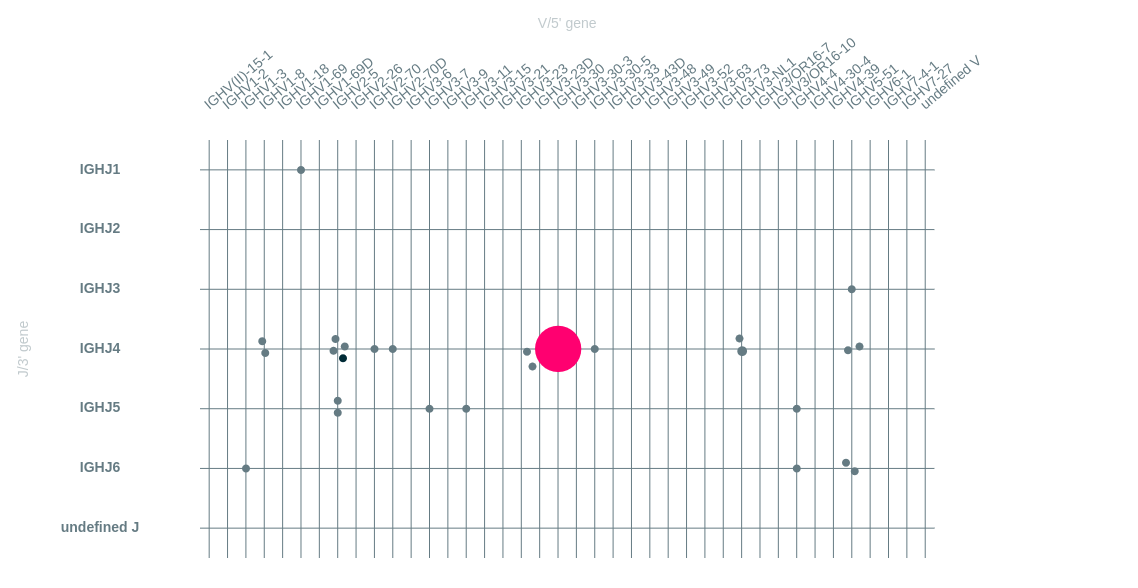
\includegraphics[width=1\textwidth]{images/diag_leader.png}
    \vspace{0.5cm}
    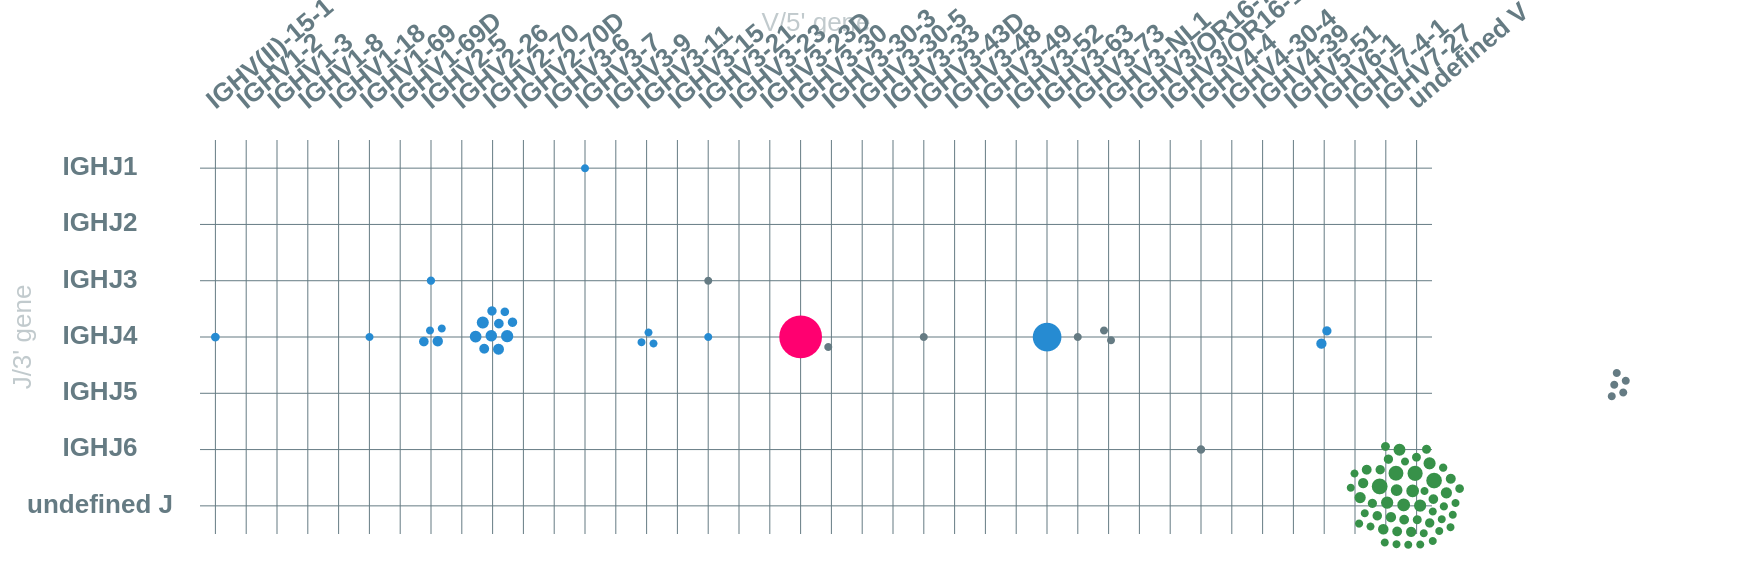
\includegraphics[width=1\textwidth]{images/diag_fr3.png}
    \caption{
        Répartition des clones identifiés en \textit{leader} (en haut) et en \gls{fr}3 (en bas) 
        pour le patient 1 au diagnostic. On observe que le \textcolor{Magenta}{clone majoritaire (en rose)} 
        en \textit{leader} est largement minoritaire en \gls{fr}3, devant les \textcolor{ProcessBlue}{nombreux clones artéfactuels en bleu}  
        et \textcolor{ForestGreen}{hors-cibles en vert}.
    }
    \label{fig:fr3-vs-leader}
\end{figure}


\section{Développements}

Un certain nombre des défis posés par le protocole de séquençage \gls{fr}3 ont ont pu être surmontés conjointement par 
des adapations techniques et bio-informatiques. Au niveau du protocole d'amplfication, une refonte complète des concentrations 
relative des différentes amorces, du protocole d'extration et des températures de \gls{pcr} ont permis d'améliorer nettement 
la qualité des données obtenues. Le cœur de cette section sera consacré au détail des approches bio-informatiques mises en place, 
nottament concernant les clones artéfactuels issus des dimères d'amorces et séquences hors-cibles 

\subsection{Séquences hors-cibles}

En ce qui concerne les artéfacts issues des dimières d'amorces, il est assez naturel que \textit{Vidjil} les identifie comme 
des réarrangements \gls{vdj} valides, comprement une section V et J. Il est par contre plus surprenant que des séquences ne comprenant 
ni gènes V ni J soient également identifiées comme des réarrangements \gls{vdj} valides. Ces séquences étant par ailleurs souvent majoritaires 
dans les premières données obtenues, pouvant représenter jusqu'à 50 \% \textit{reads} indentifiés par \textit{Vidjil}.

Lorsqu'on aligne ces séquences sur le génome humain, on observe qu'elles correspondent à diverses régions du génome, avec un aligment quasi 
parfait, à l'exception de quelques bases aux extrémités des séquences. Ces bases sont toutes identiques et correspondent à la séquence 
\C\G\T\C\T\C\C\T\C\A\G\G\T\A\A\G, ou à sa séquence complémentaire (inversée) \C\T\T\A\C\C\T\G\A\G\G\A\G\A\C\G.

Dans l'hypothèse d'une amplification non spécifique, il est possible que ces séquences correspondent à des fragments d'ammorces,
hypothèse qu'il est facile de vérifier en recherchant ces séquences dans les amorces utilisées pour l'amplification 
(\autoref{lst:bash-search-primer}).

\begin{lstlisting}[language=custombash, 
caption={Commande Bash et résultat de la recherche des séquences dans les amorces dégénérées},
label={lst:bash-search-primer},
basicstyle=\ttfamily\scriptsize]
$ grep -i --color -C 1 "CTTACCTGAGGAGACG" primers.fa
>IGH-J-A-1
caagcagaagacggcatacagatxxxxxxxxgtgactggagttcagacgtgtgctcttccgatctCTTACCTGAGGAGACGgtgacc

$ echo "CGTCTCCTCAGGTAAG" | tr 'ACGT' 'TGCA' | rev | \
        xargs -I{} grep -i --color -C 1 {} primers.fa
>IGH-J-A-1
caagcagaagacggcatacagatxxxxxxxxgtgactggagttcagacgtgtgctcttccgatctCTTACCTGAGGAGACGgtgacc

\end{lstlisting}

\subsection{Supression réversible de clonotypes}

